\documentclass[conference]{IEEEtran}
\IEEEoverridecommandlockouts
% The preceding line is only needed to identify funding in the first footnote. If that is unneeded, please comment it out.
\usepackage{cite}
\usepackage{amsmath,amssymb,amsfonts}
\usepackage{algorithm}
\usepackage{algpseudocode}
\usepackage{graphicx}
\usepackage{textcomp}
\usepackage{xcolor}
\usepackage{lipsum}

\def\BibTeX{{\rm B\kern-.05em{\sc i\kern-.025em b}\kern-.08em
    T\kern-.1667em\lower.7ex\hbox{E}\kern-.125emX}}
\begin{document}

\title{Fast and Interactive Byzantine Fault-tolerant Web Services via Session-Based Consensus Decoupling}
% \title{Session-based Consensus Simulation Layer for Interactive BFT Web Services}
% \title{Enhancing BFT Web Service Interactivity: A Layered and Session-Based Approach}
% \title{Optimizing Interactivity in BFT Web Services with Session-Based Transaction Buffering Layer}
% \title{Decoupling Interaction from Consensus: A Layered and Session-Based Architecture for BFT Web Services}
% \title{Improving User Experience in BFT Web Services Through Session-Aware Transaction Buffering}

% Keyword:
%   - session
%   - interactivity
%   - responsiveness

\author{
\IEEEauthorblockN{
    Ahmad Zaki Akmal, Azkario Rizky Pratama, and Guntur Dharma Putra\IEEEauthorrefmark{1} \\
    Universitas Gadjah Mada, Indonesia \\
    ahmad.zaki.akmal@mail.ugm.ac.id, \{azkario, gdputra\}@ugm.ac.id
    }
\thanks{\IEEEauthorrefmark{1}Corresponding author.}
}

\maketitle

\begin{abstract}
Byzantine fault-tolerant (BFT) web services provide critical integrity guarantees for distributed applications but face significant latency challenges that hinder interactive user experiences. We propose a novel two-layer architecture that addresses this fundamental tension between security and responsiveness in BFT systems. Our approach introduces a session-aware transaction buffer layer (Layer 2) that delivers immediate feedback to users through consensus simulation, while periodically committing batched operations to a fully Byzantine fault-tolerant consensus layer (Layer 1). By separating interactive operations from consensus finalization, our system achieves responsive user experiences of under 200ms, while maintaining strong BFT security guarantees. We demonstrate the efficacy of our architecture through a supply chain management implementation, where operators require both immediate feedback during multi-step workflows and tamper-proof record keeping. Our evaluation shows that our Layer 2 operations perform four times faster than the Layer 1 counterpart, while substantially preserving the end-to-end transaction integrity. Our approach enables BFT applications in domains previously considered impractical due to latency constraints, such as metaverse environments, where users require both responsive interaction and guaranteed state consistency.
\end{abstract}

\begin{IEEEkeywords}
web services, Byzantine fault tolerance, session, interactivity, responsiveness, layered architecture
\end{IEEEkeywords}

\section{Introduction}
\label{sec:introduction}

The concept of metaverse represents a shift in digital interaction, evolving beyond isolated virtual experiences toward persistent, interconnected 3D spaces where users can socialize, work, and engage in commerce~\cite{encyclopedia2010031, rony_e-commerce_2024}. The metaverse vision aligns naturally with Web3 principles, where blockchain technology enables decentralized ownership, transferable digital assets, and trustless transactions~\cite{hatami_survey_2024}. As these interconnected economies mature, enabling users to trade assets with real-world values~\cite{yang_web30_2023}, the underlying web services must evolve beyond traditional centralized architectures. Open metaverses particularly benefit from Byzantine fault tolerance due to their decentralized nature~\cite{rajawat_enhancing_2023}, ensuring consensus and transaction validity without relying on trusted intermediaries, a necessity when handling valuable digital assets in environments without central authority.

Byzantine Fault-tolerant (BFT) systems operate correctly even when up to one-third of the nodes act maliciously~\cite{lamport_byzantine_1982, castro_practical_2002}, making them crucial for metaverse applications where digital assets represent real economic value. However, current BFT web services face significant latency challenges that hinder interactive user experiences. The state-of-the-art DeWS (Decentralized Web Services) introduces approximately one second of latency for a 15-node system configuration~\cite{ramachandran_dews_2023}. Such delays create substantial friction in interactive environments where users expect near-instantaneous feedback, representing a fundamental tension between security guarantees and interactive responsiveness.

To illustrate this challenge, consider a supply chain workflow with multiple verification steps involving several stakeholders: suppliers, warehouse operators, and couriers. Each package undergoes verification, quality checks, and labeling before delivery. Warehouse operators require instant feedback during each processing step, while business management needs to ensure correctness and establish trust between stakeholders. The challenge becomes evident during high-volume periods when operators cannot afford delays waiting for consensus verification between steps, yet the business cannot compromise on creating an auditable and tamper-proof record of all activities. Similar requirements exist in healthcare, financial services, e-government, and metaverse environments, where participants need both high responsiveness during operations and guaranteed integrity of the final record. In these multi-step workflows, even small delays at each verification stage compound exponentially, potentially bringing operations to a standstill while participants wait for consensus confirmation. This operational bottleneck not only impacts productivity but also undermines user adoption of otherwise secure distributed systems.

Current approaches to this challenge typically force a binary choice between security and performance. Traditional centralized systems achieve low latency but sacrifice fault tolerance and require trusted authorities, making them unsuitable for cross-organizational workflows or decentralized environments. Conversely, existing BFT systems prioritize security but impose consensus overhead on every operation, resulting in cumulative delays that render them impractical for interactive applications. This fundamental limitation has restricted BFT adoption to scenarios where occasional high latency is acceptable, leaving a significant gap for applications requiring both security guarantees and responsive user interactions.

In this paper, we propose a two-layered web service architecture to address the latency challenge while maintaining Byzantine fault tolerance. The first layer (L1) conducts full BFT consensus across a distributed network of nodes, while the second layer (L2) implements a novel session-based transaction buffer that provides immediate feedback to users through consensus simulation. We introduce the concept of \textit{sessions}, where related operations are grouped and processed through the responsive L2 simulation before being committed as a batch to the more secure but slower L1 consensus. This approach significantly reduces both perceived latency and the frequency of slower L1 consensus operations.

Our work offers these key contributions:
\begin{itemize}
    \item We introduce \textit{a two-layer architecture for BFT web services} that separates interactive simulation from consensus finalization, enabling responsive user experiences while maintaining security guarantees.
    
    \item We develop \textit{a transaction buffering mechanism} that groups related operations into sessions, simulates their execution with up-to-date state data, and commits them as atomic units, reducing perceived latency while preserving transactional integrity.
    
    \item We provide \textit{a fully functional proof-of-concept} for our proposed solution through a supply chain scenario that demonstrates its practical feasibility along with a detailed performance evaluation.
\end{itemize}

The remainder of this paper is organized as follows. Section~\ref{sec:related-work} reviews related work on BFT systems and Layer 2 technologies. Section~\ref{sec:system-model} presents our system architecture, while Section~\ref{sec:implementation} describes our implementation details. We conclude our work in Section~\ref{sec:conclusion}.

\section{Related Work}
\label{sec:related-work}

Byzantine Fault Tolerance (BFT) addresses the challenge of maintaining system correctness despite arbitrary failures or malicious behavior in some components. In web services, BFT is particularly important when operations span multiple organizations with different trust boundaries~\cite{lamport_byzantine_1982}.

Practical Byzantine Fault Tolerance (PBFT)~\cite{castro_practical_2002} made BFT implementations feasible by reducing communication complexity from exponential to polynomial. Zyzzyva~\cite{kotla_zyzzyva_2008} further improves performance by lowering latency, involving clients to assist in validations. However, PBFT, Zyzzyva, and their derivatives still face scalability challenges, particularly in high-throughput interactive applications.

Several approaches have applied BFT concepts to web services, including Thema~\cite{merideth_thema_2005}, BFT-WS~\cite{zhao_bft-ws_2007}, WebBFT~\cite{berger_webbft_2018}, and the most recent, DeWS~\cite{ramachandran_dews_2023}. Thema and BFT-WS implement Byzantine fault tolerance for Web Services while maintaining compatibility with standard SOAP and WSDL protocols, but they rely on centralized middleware architectures, which can become potential bottlenecks or single points of failure. WebBFT later improved on these ideas by making BFT services accessible to browser-based clients. It supported real-time collaborative features like publish-subscribe updates and worked with modern web technologies such as WebSockets~\cite{berger_webbft_2018}. Despite these advances, WebBFT faced several challenges. It introduced noticeable performance overhead from browser-side cryptography and JSON handling, and was vulnerable to denial-of-service attacks caused by malicious clients triggering repeated leader changes. These issues limited its scalability and robustness in adversarial environments.

A key similarity among these earlier efforts is that they achieve BFT by reaching consensus on the computation result of a single web server or through the inclusion of centralized components, thus lacking full computation replication across nodes. In contrast, Ramachandran et al. argue that replicating the complete computation at each node is necessary to ensure safety in the presence of Byzantine faults, a principle that underpins their design of DeWS~\cite{ramachandran_dews_2023}.

DeWS implements a brand new interaction model: \textit{request-compute-consensus-log-response}. All operations undergo replication and consensus validation before responses are returned to clients, ensuring that responses are agreed upon by a quorum of nodes. This approach provides strong integrity and auditability guarantees but introduces significant latency—approximately 935ms with 15 nodes even in a Docker container network, which represents an ideal environment compared to real-world deployments~\cite{ramachandran_dews_2023}. This latency creates a fundamental tension between Byzantine fault tolerance and interactivity, making DeWS challenging to apply in scenarios requiring frequent user interactions or real-time feedback.

Layer 2 blockchain solutions address similar scalability challenges by offloading transaction processing from the main chain. Techniques such as rollups and sidechains enable higher throughput and lower latency while maintaining security by periodically anchoring state to the layer 1 chain~\cite{mandal_investigating_2023, thibault_blockchain_2022}.

Session management, the grouping of related operations into logical units, has been explored in distributed systems primarily for user authentication and state tracking~\cite{calzavara_measuring_2021}. However, its potential for optimizing consensus operations remains largely unexplored in BFT web services.

\begin{figure}[t]
    \centering
    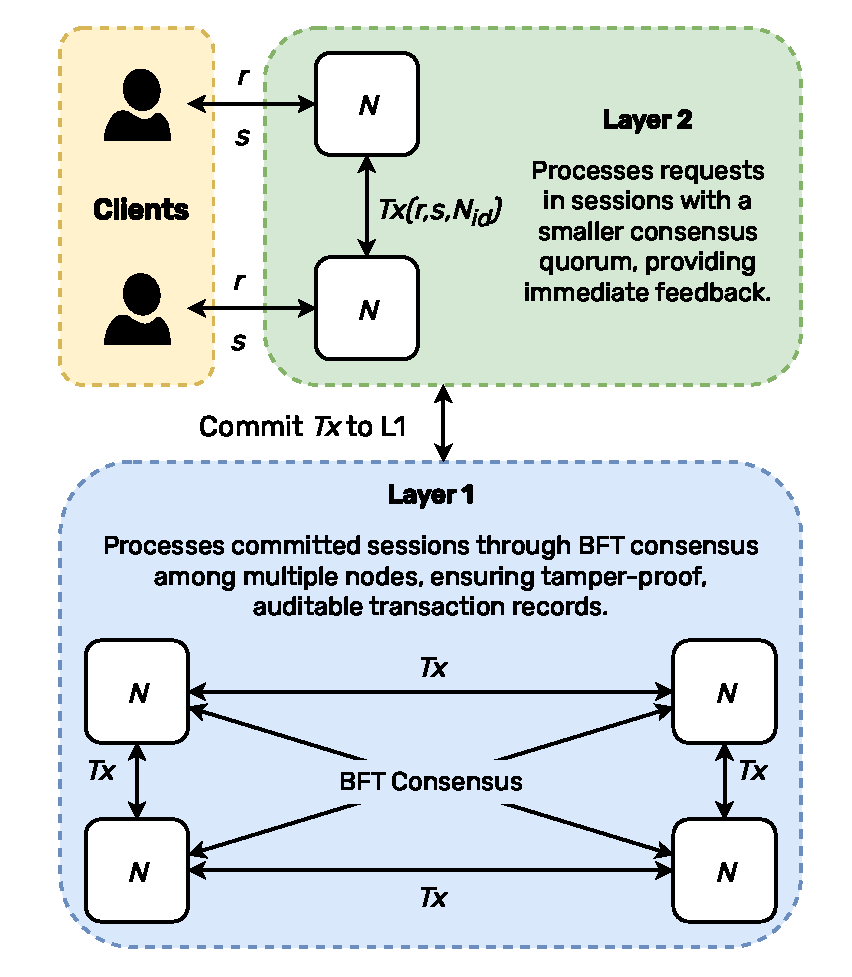
\includegraphics[width=0.85\linewidth]{figure/Thesis Diagrams-V5. Layer 2 System Architecture .drawio.pdf}
    \caption{Our two-layer architecture for BFT web services, showing client interactions with Layer 2 nodes and eventual session commitment to the Layer 1 BFT consensus network.
    % This design balances immediate response times with strong security guarantees, enabling both interactive performance and Byzantine fault tolerance.
    }
    \label{fig:system_model}
\end{figure}

While these previous works have advanced Byzantine fault tolerance in web services, they collectively fail to address the fundamental trade-off between interactive responsiveness and strong BFT guarantees. The absence of a solution that maintains both low-latency interactivity and strong BFT guarantees represents a significant gap in the literature. Our two-layer architecture directly addresses this gap by separating the concerns of immediate feedback and consensus validation, enabling responsive user experiences without sacrificing the integrity guarantees of Byzantine fault tolerance.

\section{System Model and Architecture}
\label{sec:system-model}

In this section, we describe our proposed solution that addresses the latency challenges in distributed web services while maintaining Byzantine fault tolerance.


% \begin{figure}
%     \centering
%     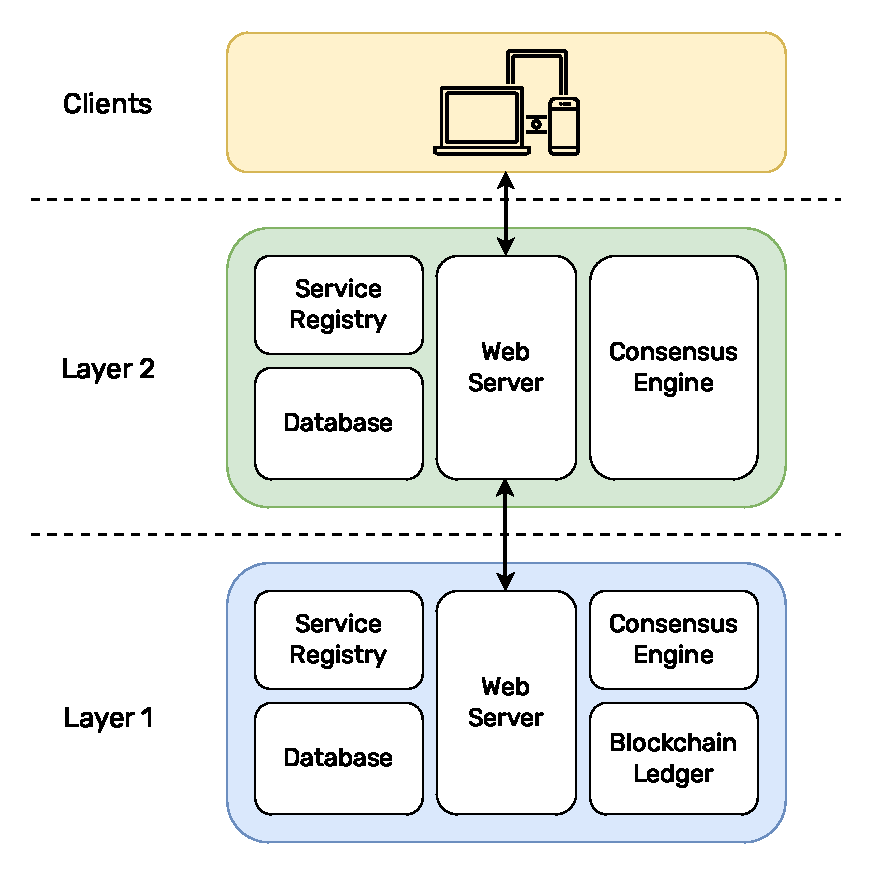
\includegraphics[width=1\linewidth]{figure/layer_diagram.drawio.pdf}
%     \caption{Layer overview of the system, showing detailed view of each layer's components}
%     \label{fig:system_layers}
% \end{figure}


% \subsection{System Components}
% \label{subsec:definitions}

% Our model consists of two distinct layers: Layer 2 (L2) for transaction simulation and Layer 1 (L1) for Byzantine fault-tolerant consensus. These layers work together to provide low-latency interactions during workflow execution while ensuring final state consistency through consensus. Below we describe the definition of our system components in more detail.

% \subsubsection{\textbf{Node}}
% A node $N$ is the fundamental building block of the distributed network. In our design, each node consists of a web server, a consensus engine, and a database. Nodes connect with each other, forming the network of a layer.

% \begin{figure*}[!t]
%     \centering
%     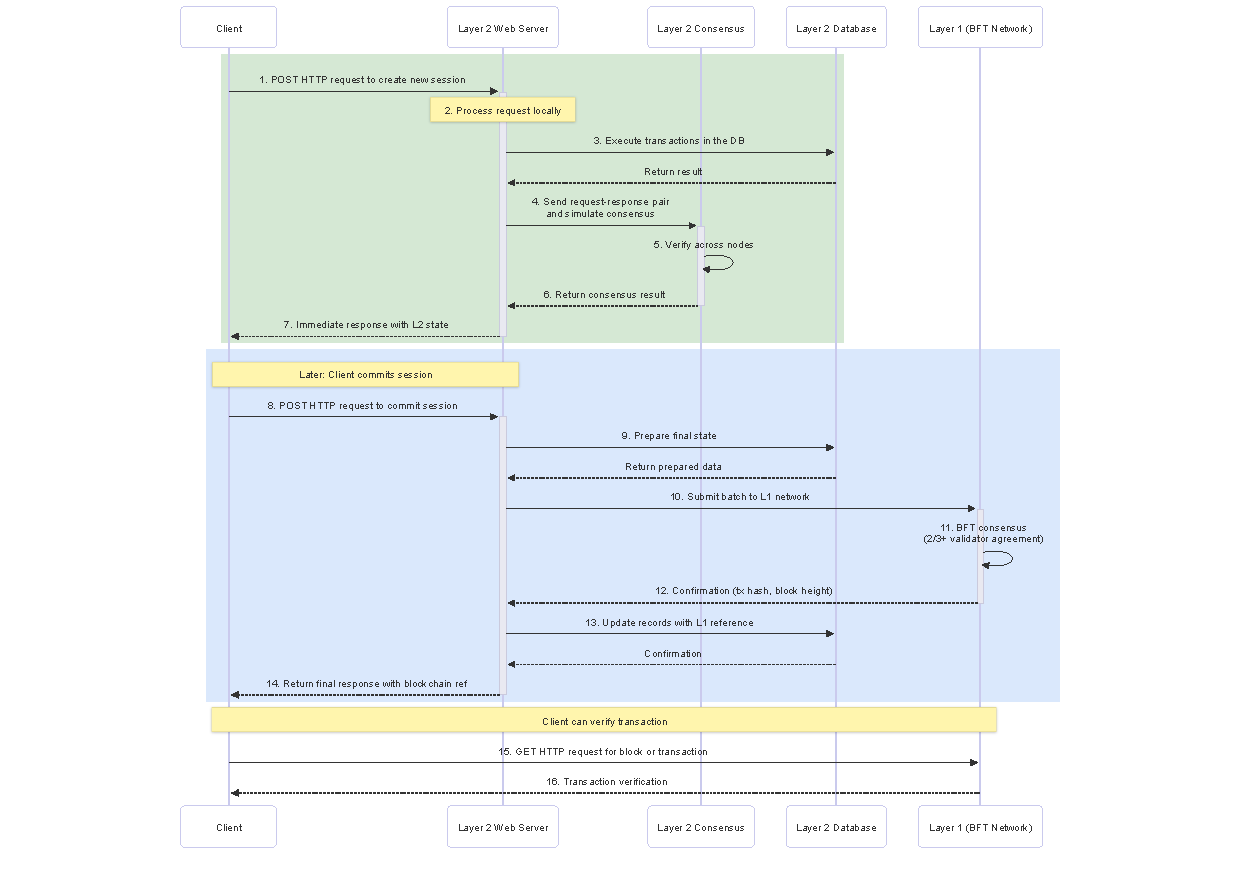
\includegraphics[width=.9\textwidth]{figure/editor___mermaid_chart-2025-05-11-115647.pdf}
%     \caption{Sequence diagram illustrating the two-layer transaction processing flow. The workflow begins with client session creation handled locally by L2 (marked green), providing immediate responses.
%     Transactions are then committed to the L1 (marked blue), requiring validator agreement before confirmation.}
%     \label{fig:system_flow}
% \end{figure*}

% \subsubsection{\textbf{Service Handler}}
% A Service Handler is a function that processes a specific type of HTTP request, identified by its method and path. Formally, for a request $r$, a service handler is a function $H: R \rightarrow S$ that maps from the request domain $R$ to the response domain $S$. The function may also signal exceptional conditions through implementation-specific mechanisms. Service handlers encapsulate endpoint-specific functionality, allowing the system to maintain separation between routing and business logic.

% \subsubsection{\textbf{Service Registry}}
% The Service Registry is a management component that maintains a mapping between API routes (HTTP method and path combinations) and their corresponding service handlers. It can be represented as $\mathcal{R} = \{(m_i, p_i) \mapsto H_i\}$ where $m_i$ is an HTTP method, $p_i$ is a URL path pattern, and $H_i$ is the associated handler function. The registry provides a lookup function $\mathcal{L}(m, p) \rightarrow H$ that maps an incoming request's method $m$ and path $p$ to the appropriate handler $H$. By centralizing route management, the Service Registry enables the system to apply consistent processing between the web server and the consensus replication.

% \subsubsection{\textbf{Transaction}}
% A Transaction $Tx = (r, s, N_{id})$ consists of a request $r$, its associated response $s$ generated by a service handler, and the identifier $N_{id}$ of the originating node. Transactions are the fundamental unit of consensus in the system, allowing nodes to verify whether a given request produces the expected response according to the business rules encoded in service handlers. A transaction is considered valid when it meets two conditions: (1) the response was generated by applying the correct service handler to the request, and (2) a majority of nodes in the network have independently verified that applying the same service handler to the request produces an identical response. This verification process ensures that Byzantine nodes cannot tamper with transaction results. Otherwise, it is marked as an invalid transaction.

% \subsubsection{\textbf{Transaction Originator}}
% The Transaction Originator is the node that first receives a client request, processes it using the appropriate service handler, and creates the initial transaction with its identifier $N_{id}$. This node is responsible for broadcasting the transaction to other nodes in the network to begin the consensus process. The originator's node ID is included in the transaction to maintain provenance and accountability in the network.

% \subsubsection{\textbf{BFT Consensus}}
% Byzantine Fault Tolerant (BFT) Consensus is a distributed agreement process that can tolerate Byzantine faults—nodes that may behave arbitrarily or maliciously. In our system, BFT consensus requires a minimum of $4$ nodes and achieves agreement when at least $\lceil \frac{2n+1}{3} \rceil$ nodes (where $n$ is the total number of nodes) validate a transaction. This ensures system correctness even if up to $\lfloor \frac{n-1}{3} \rfloor$ nodes are Byzantine. The BFT consensus layer provides strong finality guarantees but introduces latency proportional to network size.

% \subsubsection{\textbf{Simulation Consensus}}
% Simulation Consensus is a lightweight agreement process used in Layer 2 that prioritizes responsiveness over Byzantine fault tolerance. It mimics the validation logic of the main BFT consensus but operates with relaxed participation requirements. This approach enables interactive, low-latency responses during multi-step workflows while maintaining consistent rule application. Transactions reaching simulation consensus are stored in a buffer and can later be committed to the BFT consensus layer as a batch, providing eventual Byzantine fault tolerance while significantly improving response times.

\subsection{System Architecture}
Figure~\ref{fig:system_model} illustrates the architecture of our proposed system. The system employs a dual-layer approach, each consisting of interconnected nodes with specific responsibilities. As shown in the diagram, every node in both layers incorporates these core components:

\begin{itemize}
\item Consensus Engine: Manages all consensus-related functions, including transaction verification, BFT consensus execution, block commitment, and ledger storage. This component also handles peer-to-peer (P2P) communication with other nodes within the same layer.
\item Web Server: Provides an HTTP interface exposing endpoints that enable clients to interact with the system through standardized APIs.
\item Service Registry: This component maps API routes to their corresponding handlers.
\item Database: Stores session data, transaction history, and application-specific information required for system operation.
\end{itemize}

These components work together to form a cohesive system that achieves both Byzantine fault tolerance and responsive performance.

\subsection{Layer 1 (L1): Byzantine Fault-Tolerant Foundation}

The first layer implements a design inspired by DeWS, where each node represents a domain operated by a distinct organization participating in the application ecosystem~\cite{ramachandran_dews_2023}. Unlike traditional BFT research that focuses on abstract state machine replication, our approach necessarily integrates business verification with consensus processes—a design choice required for cross-organizational applications where business rule enforcement cannot rely on trusted intermediaries.

L1 serves as the primary foundation for BFT by implementing full BFT consensus protocols. Nodes in L1 maintain identical service registries and execute consensus only when receiving commit requests from L2 nodes. Each validator independently verifies transaction validity by applying the same service handler as the transaction originator and comparing response equivalence.

To satisfy BFT requirements, L1 must contain at least four nodes, which is the minimum necessary to tolerate one Byzantine fault, following the standard rule that a BFT system requires at least $3f+1$ nodes to tolerate $f$ Byzantine faults. In addition to the standard node components, L1 nodes maintain an immutable blockchain ledger, providing tamper-proof storage of confirmed transactions.

\begin{algorithm}[t]
\caption{Unified Consensus Process (Both L1 and L2)}
\label{algorithm:validate-tx-process-proposal}
\begin{algorithmic}[1]

\Procedure{ValidateTransaction}{transaction}
    \State \textbf{Layer 1:} Verify transaction is well-formed and properly signed
    \State \textbf{Layer 2:} Check transaction against session state and business rules
    
    \State Decrypt and parse transaction content
    
    \If{transaction format is invalid}
        \State \Return FALSE \Comment{Malformed transaction}
    \EndIf
    
    \If{transaction violates state constraints}
        \State \Return FALSE \Comment{Transaction is invalid}
    \EndIf
    
    \State Execute transaction against current state
    % \State Record response and state changes
    
    \State \Return TRUE \Comment{Transaction is valid}
\EndProcedure


\Procedure{ProcessProposal}{proposedBlock}
    \State \textbf{Layer 1:} Validators independently execute transactions and compare results
    \State \textbf{Layer 2:} Simulates validation by re-executing operations against local state
    \If{results from execution differ from proposed results}
        \State \Return REJECT \Comment{Byzantine behavior detected}
    \Else
        \State \Return ACCEPT \Comment{Proposed transactions is valid}
\EndIf
\EndProcedure

% \Procedure{FinalizeBlock}{acceptedBlock}
%     \State \textbf{Layer 1:} Update blockchain state with transaction results
%     \State \textbf{Layer 2:} Update session state with L1 consensus results
%     \State \Return Block results with cryptographic proof
% \EndProcedure

% \Procedure{Commit}{}
%     \State \textbf{Layer 1:} Persist block and state changes to blockchain
%     \State \textbf{Layer 2:} Mark session as committed with blockchain reference
%     \State \Return Consensus success acknowledgment
% \EndProcedure

\end{algorithmic}
\end{algorithm}

\subsection{Layer 2 (L2): Interactive Transaction Layer}

The second layer represents the core innovation of our architecture. L2 functions as a transaction buffer, performing simulation consensus and batching operations for efficient commitment to L1. Each node in L2 employs the same service registry and service handlers both in the web server and consensus components.
Unlike L1, this layer is not required to fulfill the strict BFT node count requirements; instead, it inherits fault tolerance properties from the underlying L1 network.% When a node receives a client request, it becomes the \textit{transaction originator} for that operation, creating a \textit{transaction} after generating a response.

The separation between layers enables L2 to prioritize fast responsiveness over native BFT, effectively optimizing system performance for interactive applications while still validating transactions according to system rules. Furthermore, L2 is designed to operate with a minimal number of nodes, allowing consensus simulation to complete faster and reducing the latency introduced during transaction processing.

\subsection{System Flow}

% Figure~\ref{fig:system_flow} illustrates the complete transaction lifecycle in our two-layer architecture.
The process begins when a client sends a request to initiate a new session with a Layer 2 node. The receiving node, becoming the transaction originator, processes the request by using its service registry to identify the appropriate service handler. The handler processes the request locally and stores the session in the node's database. After processing, the service handler generates a response $s$, which together with the original request $r$ and the node's identifier $N_{id}$ forms a transaction $Tx(r, s, N_{id})$.

% L2=1 Endpoints & Total Workflow
\begin{figure}[t]
    \centering
    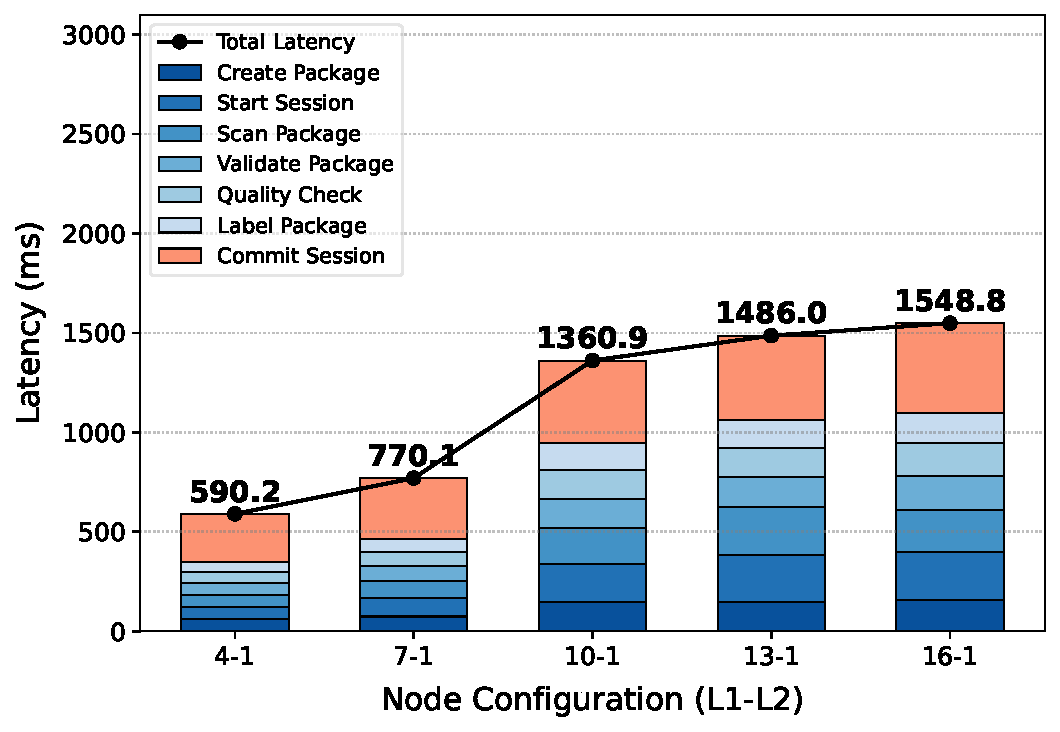
\includegraphics[width=1\linewidth]{figure/ieee_stacked_latency_l1_l2_1.pdf}
    \caption{Detailed endpoint latency breakdown for configurations with a single L2 node, showing individual endpoint contributions to total workflow latency.}
    \label{fig:stacked-endpoints-l2-1}
\end{figure}

The transaction originator forwards this transaction to the L2 consensus layer, which performs simulation consensus by replicating the operation across other L2 nodes. As shown in Algorithm~\ref{algorithm:validate-tx-process-proposal}, each participating node processes the request through its own service registry and service handlers to verify response consistency. During the Process Proposal phase, nodes execute transactions independently and reject proposals if the results differ, detecting Byzantine behavior. If the deployment has only a single L2 node, it still executes consensus validation steps internally to ensure compliance with network rules.

% L2=1 trend
% \begin{figure}[t]
%     \centering
%     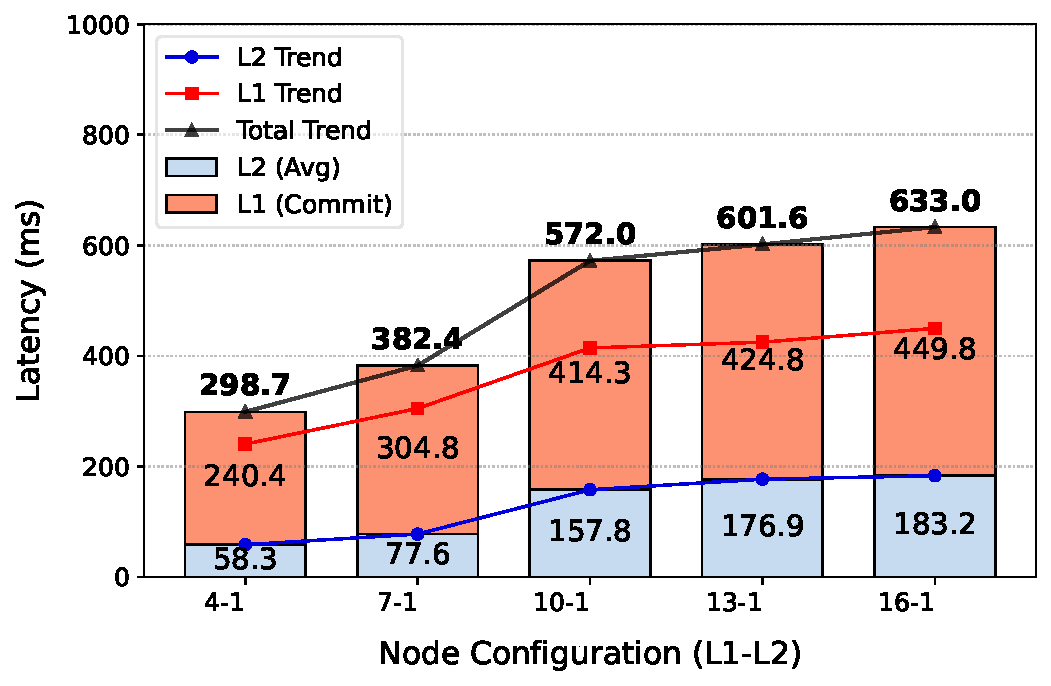
\includegraphics[width=1\linewidth]{figure/bft_l1_l2_comparison_ieee_l2_1.pdf}
%     \caption{Latency analysis of BFT node configurations with a single Layer 2 node, showing the trend of L2 operation latency, L1 commit latency, and total workflow latency across various L1 node configurations.}
%     \label{fig:average_comparison_l1_l2_1}
% \end{figure}

After session creation, clients can execute a series of related operations within the same session context. Each subsequent request follows the same processing pattern as the initial session creation, with the important distinction that each operation is validated against the session's current state, following the validation logic in Algorithm~\ref{algorithm:validate-tx-process-proposal}.

The L1 layer operates a full BFT consensus mechanism. Similar to the L2 process, the transaction originator on L1 first replicates the complete session across validators. It generates a transaction containing all operations and submits it to the L1 consensus layer. The BFT consensus algorithm requires validation from at least $\lceil \frac{2n+1}{3} \rceil$ nodes to consider the transaction valid; otherwise, it is rejected.

Upon reaching consensus, the L1 network returns the result to the L2 node along with blockchain reference data such as block height and transaction hash. The L2 node then updates the session status accordingly, propagates this update to other L2 peers, and delivers the final result to the client. For verification purposes, clients can query transaction status either through an L2 node or directly from the L1 network, depending on the implementation.

This two-layer approach combines the immediate responsiveness of simulation consensus with the security guarantees of BFT consensus, creating a system that is both interactive and trustworthy.

% L2=2 Endpoints & Total Workflow
\begin{figure}[t]
    \centering
    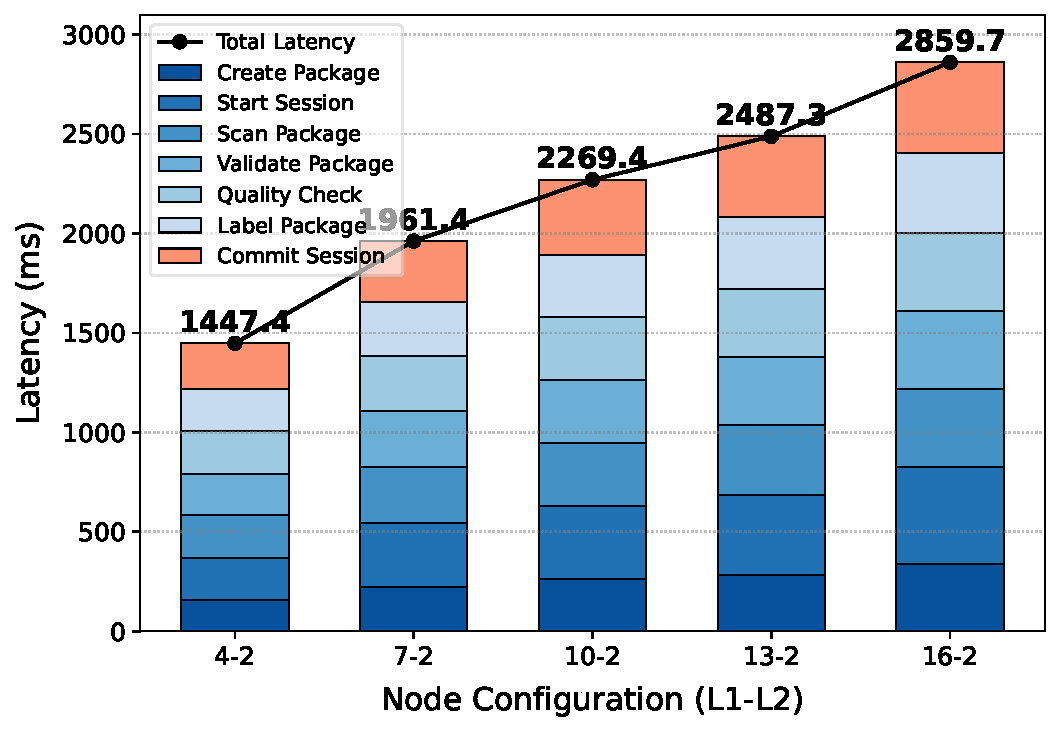
\includegraphics[width=1\linewidth]{figure/ieee_stacked_latency_l1_l2_2.pdf}
    \caption{Detailed endpoint latency breakdown for configurations with dual L2 nodes, showing individual endpoint contributions to total workflow latency.}
    \label{fig:stacked-endpoints-l2-2}
\end{figure}

\section{Performance Evaluation}
\label{sec:implementation}

% \subsection{Use Case: Supply Chain Management}
Our proof-of-concept implementation demonstrates a supply chain management system that represents an ideal scenario where both high responsiveness and strong security guarantees are the required attributes. Supply chain operations demand fast and interactive processing to maintain throughput while simultaneously requiring tamper resistance to prevent fraud across organizational boundaries. As such, our use case demonstrates the need for session fault tolerance, step-by-step feedback without premature commitment, and a tamper-proof audit trail. The implemented workflow consists of five sequential stages: 
(1) session initiation, where an operator begins processing a package; (2) package scanning, which identifies and retrieves expected contents; 
(3) validation of the package's digital signature to authenticate its origin; 
(4) quality control inspection; and 
(5) shipping label generation and courier assignment. Once completed, the entire session can be committed as an atomic unit to the Byzantine fault-tolerant L1, demonstrating how our dual-consensus architecture effectively balances responsive user experience with strong security guarantees in multi-step business processes. It should be noted that while this workflow represents a simplified version of real-world supply chain operations, it captures the essential characteristics and challenges that our system is designed to address.

\subsection{Proof-of-Concept Implementation}

% \begin{table}[t]
% \caption{Summary of Formal Notations}
% \label{tab:formal_notations}
% \centering
% \begin{tabular}{|l|p{3.5cm}|p{5.5cm}|}
% \hline
% \textbf{Notation} & \textbf{Description} & \textbf{Parameters/Properties} \\
% \hline
% $N$ & Node & A fundamental building block consisting of a web server, consensus engine, and database \\
% \hline
% $H : R \rightarrow S$ & Service Handler & A function mapping from request domain $R$ to response domain $S$ \\
% \hline
% $R = \{(m_i, p_i) \mapsto H_i\}$ & Service Registry & A mapping from HTTP method $m_i$ and path $p_i$ to handler $H_i$ \\
% \hline
% $L(m, p) \rightarrow H$ & Lookup Function & Maps request method $m$ and path $p$ to the appropriate handler $H$ \\
% \hline
% $Tx = (r, s, N_{id})$ & Transaction & Consists of request $r$, response $s$, and originator node ID $N_{id}$ \\
% \hline
% $N_{id}$ & Transaction Originator ID & Identifier of the node that first receives a client request \\
% \hline
% $\lceil\frac{2n+1}{3}\rceil$ & BFT Consensus Threshold & Minimum number of nodes required for agreement (where $n$ is total nodes) \\
% \hline
% $\lfloor\frac{n-1}{3}\rfloor$ & Byzantine Fault Tolerance & Maximum number of Byzantine nodes that can be tolerated \\
% \hline
% \end{tabular}
% \end{table}

We utilized CometBFT as the consensus engine, providing customizable and robust BFT using the Tendermint consensus algorithm~\cite{buchman_latest_2019, buchman_revisiting_2022} through its \textit{Application BlockChain Interface} (ABCI). We implemented both the web server and service registry components in Go programming language to ensure optimal interoperability with CometBFT's native codebase.

Our primary goal is to enhance interactivity and responsiveness through the L2 implementation, so our evaluation focuses primarily on latency metrics. We define latency as the time it takes from request initiation to response reception, calculated as $t_{\text{res}} - t_{\text{req}}$, where $t_{\text{res}}$ represents the response reception timestamp and $t_{\text{req}}$ represents the request initiation timestamp.

% L1 vs L2 comparison (L2 = 1)
\begin{figure}[t]
    \centering
    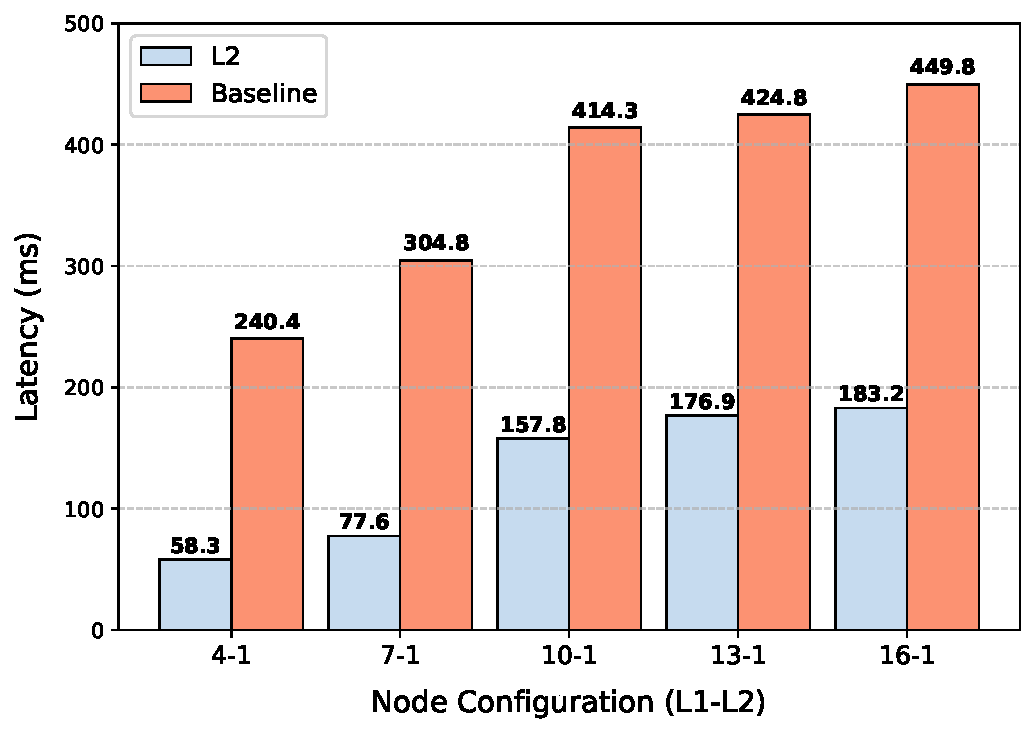
\includegraphics[width=1\linewidth]{figure/l1_vs_l2_comparison_l2_1.pdf}
    \caption{Response time comparison between L1 commitment operations and L2 simulation with L2=1 configurations, showing the significant decrease in latency at about 2.4-4.1× faster.}
    \label{fig:baseline-comparison-l2-1}
\end{figure}

We conducted comprehensive measurements for each step in the workflow sequence: from session creation through to blockchain commitment. To facilitate multiple test iterations, we implemented a package creation step that generates unique package identifiers for each test run. This approach enabled us to execute measurements systematically across varying node configurations. For each complete workflow, we performed 100 iterations to ensure statistical significance and reliability of our results.

For clarity in presenting our results, we use the notation $L1$-$L2$, where $L1$ represents the number of nodes in the BFT Layer 1 network and $L2$ represents the number of nodes in the simulation Layer 2 network. We systematically tested configurations with 1 and 2 L2 nodes while varying L1 nodes across five different cluster sizes: 4, 7, 10, 13, and 16. These specific node counts were selected to represent increasing Byzantine fault tolerance thresholds from 1 to 5, calculated according to the standard formula $n = 3f+1$~\cite{lamport_byzantine_1982}, where $n$ is the total number of nodes and $f$ is the number of tolerable Byzantine faults.

% The benchmarking framework was implemented as a standalone Go application that records performance metrics in CSV format. We then processed this data using Python to generate visualizations that highlight the performance characteristics across different system configurations.

\subsection{Experimental Results}

Our evaluation results demonstrate the significant performance advantages of the L2 session batching approach across various BFT cluster configurations.

For configurations with a single L2 node, we observed clear performance patterns as the number of L1 nodes increased. L2 operations (Create Package, Start Session, Scan Package, Validate Package, Quality Check, and Label Package) maintained relatively low latencies even as the BFT cluster size grew. Figure~\ref{fig:stacked-endpoints-l2-1} provides a detailed breakdown of individual endpoint latencies across all tested configurations with a single L2 node. The complete workflow latency increased from 590.2ms with the 4-1 configuration to 1548.8ms with the 16-1 configuration. This increase is primarily attributable to the growing complexity of achieving consensus across larger BFT networks, where additional network communication and validation steps are required for each additional node.

% L1 vs L2 comparison (L2 = 2)
\begin{figure}[t]
    \centering
    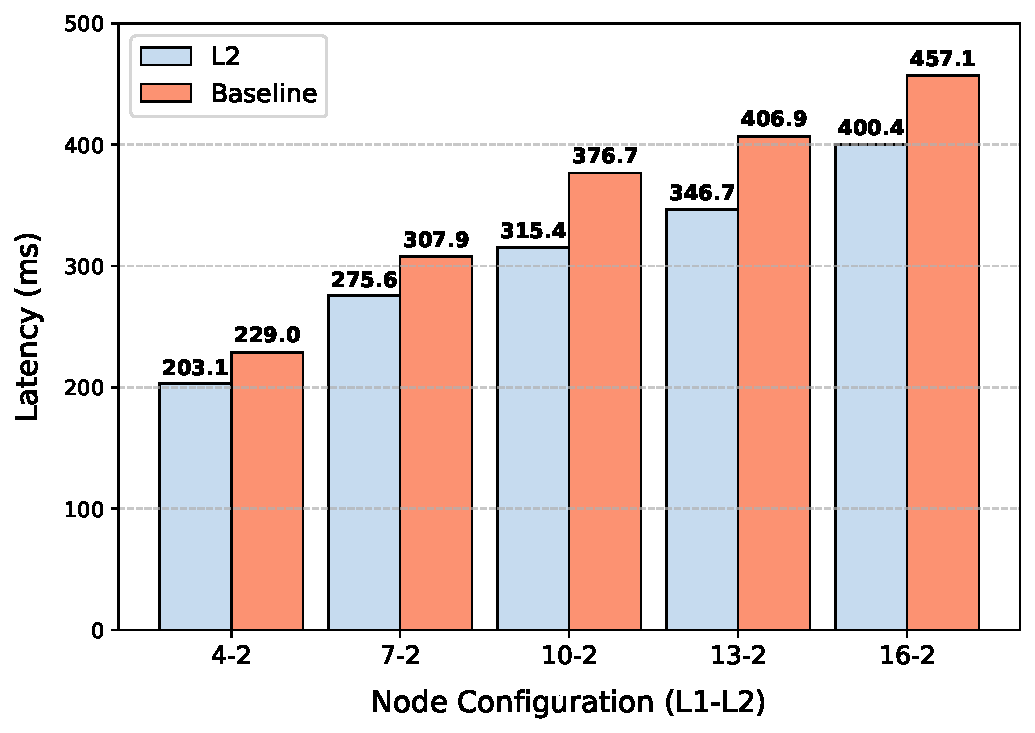
\includegraphics[width=1\linewidth]{figure/l1_vs_l2_comparison_l2_2.pdf}
    \caption{Response time comparison between L1 consensus commit operations and L2 simulation with L2=2 configurations, showing reduced performance advantages due to coordination overhead between dual L2 nodes.}
    \label{fig:baseline-comparison-l2-2}
\end{figure}

To better represent realistic consensus simulation, we tested configurations with two L2 nodes. Adding a second L2 node introduces additional coordination overhead but provides a more robust simulation environment. The endpoint-specific breakdown shows that complete workflow execution time ranges from 1447.4ms with the 4-2 configuration to 2859.7ms with the 16-2 configuration. This significant increase reflects the added complexity of coordinating two L2 nodes while simultaneously scaling the BFT L1 cluster, where inter-node communication overhead becomes more pronounced.

The direct performance comparison between L1 and L2 operations provides clear evidence of our approach's effectiveness. Looking at the comparison in Figure~\ref{fig:baseline-comparison-l2-1}, individual L2 operations averaged 58.3ms with the 4-1 configuration compared to 240.4ms for L1 consensus operations, while with the 16-1 configuration, L2 operations averaged 183.2ms compared to 449.8ms for L1 operations. Single L2 node configurations demonstrate a significant latency decrease, with L2 operations approximately 2.4 to 4.1 times faster than L1 commits across all tested cluster sizes. The performance improvement is most pronounced in smaller configurations (4.1× faster for 4-1) and remains substantial even with larger clusters (2.4× faster for 16-1).

In contrast, Figure~\ref{fig:baseline-comparison-l2-2} reveals that dual L2 node configurations show markedly reduced performance advantages due to coordination overhead between the two L2 nodes. With the 4-2 configuration, L2 operations averaged 203.1ms compared to 229.0ms for L1 operations, while scaling to the 16-2 configuration increased L2 operation latency to 400.4ms compared to 457.1ms for L1 operations. The performance improvement drops to only 1.1 to 1.2 times faster than L1 commits, with L2 latency approaching L1 latency across all configurations. This demonstrates that the coordination overhead between dual L2 nodes nearly eliminates the speed benefits of the L2 layer, making single L2 configurations significantly more effective for performance-oriented applications.

The experimental results validate our two-layer approach: Layer 2 operations consistently achieve sub-second latencies suitable for interactive use, while the more expensive BFT consensus operations are consolidated into a single commit phase.
% Even with a 16-node BFT cluster, the interactive L2 operations remain highly responsive, consistently completing in under 200ms across all configurations tested.
The substantial improvement in responsiveness enables interactive workflows that would otherwise be impractical with direct L1 consensus for each operation.
While the latencies we observed are higher than those reported for traditional \textit{request-compute-response} operations in DeWS (approximately 16-18ms for basic POST/GET operations)~\cite{ramachandran_dews_2023}, the increased responsiveness in complex multi-step workflows justifies this trade-off. Our approach provides significant benefits in terms of session management, state consistency, and interactive user experience across the two-layer architecture.

Our findings suggest that smaller L1 configurations with a single L2 node offer the best balance of performance and fault tolerance for most applications. However, for scenarios requiring higher Byzantine fault tolerance thresholds, configurations with 10 to 16 L1 nodes remain viable, with total workflow latencies still acceptable for supply chain and similar applications. The dual L2 node configurations, while theoretically providing more accurate simulation, introduce significantly higher latencies without proportional improvements in L2 operation responsiveness. This suggests that for applications prioritizing performance, either a single L2 node or direct L1 operations would be preferable to a multi-node L2 setup, as the added complexity does not yield substantial benefits in our tested scenarios.

\section{Conclusion}
\label{sec:conclusion}
This paper presented a two-layer architecture with a session-aware transaction buffer that addressed the challenge of providing interactive experiences in Byzantine fault-tolerant (BFT) web services. Our approach decoupled latency-sensitive operations from BFT consensus processes, maintaining sub-200ms response times for interactive operations even with 16-node BFT clusters. By buffering operations and deferring consensus until session completion, we achieved both the responsiveness needed for modern applications and the security guarantees of Byzantine fault tolerance. Our approach opened possibilities for BFT systems in domains previously impractical due to latency constraints, particularly for multi-step workflows like supply chain management.

\section*{Acknowledgment}
\noindent This work was supported by Hibah Penelitian Fundamental (PFR), Ministry of Higher Education, Science, and Technology Indonesia, grant number 048/E5/PG.02.00.PL/2024 - 2679/UN1/DITLIT/PT.01.03/2024.

% ==========================================

% \section{Ease of Use}

% \subsection{Maintaining the Integrity of the Specifications}

% The IEEEtran class file is used to format your paper and style the text. All margins, 
% column widths, line spaces, and text fonts are prescribed; please do not 
% alter them. You may note peculiarities. For example, the head margin
% measures proportionately more than is customary. This measurement 
% and others are deliberate, using specifications that anticipate your paper 
% as one part of the entire proceedings, and not as an independent document. 
% Please do not revise any of the current designations.

% \section{Prepare Your Paper Before Styling}
% Before you begin to format your paper, first write and save the content as a 
% separate text file. Complete all content and organizational editing before 
% formatting. Please note sections \ref{AA}--\ref{SCM} below for more information on 
% proofreading, spelling and grammar.

% Keep your text and graphic files separate until after the text has been 
% formatted and styled. Do not number text heads---{\LaTeX} will do that 
% for you.

% \subsection{Abbreviations and Acronyms}\label{AA}
% Define abbreviations and acronyms the first time they are used in the text, 
% even after they have been defined in the abstract. Abbreviations such as 
% IEEE, SI, MKS, CGS, ac, dc, and rms do not have to be defined. Do not use 
% abbreviations in the title or heads unless they are unavoidable.

% \subsection{Units}
% \begin{itemize}
% \item Use either SI (MKS) or CGS as primary units. (SI units are encouraged.) English units may be used as secondary units (in parentheses). An exception would be the use of English units as identifiers in trade, such as ``3.5-inch disk drive''.
% \item Avoid combining SI and CGS units, such as current in amperes and magnetic field in oersteds. This often leads to confusion because equations do not balance dimensionally. If you must use mixed units, clearly state the units for each quantity that you use in an equation.
% \item Do not mix complete spellings and abbreviations of units: ``Wb/m\textsuperscript{2}'' or ``webers per square meter'', not ``webers/m\textsuperscript{2}''. Spell out units when they appear in text: ``. . . a few henries'', not ``. . . a few H''.
% \item Use a zero before decimal points: ``0.25'', not ``.25''. Use ``cm\textsuperscript{3}'', not ``cc''.)
% \end{itemize}

% \subsection{Equations}
% Number equations consecutively. To make your 
% equations more compact, you may use the solidus (~/~), the exp function, or 
% appropriate exponents. Italicize Roman symbols for quantities and variables, 
% but not Greek symbols. Use a long dash rather than a hyphen for a minus 
% sign. Punctuate equations with commas or periods when they are part of a 
% sentence, as in:
% \begin{equation}
% a+b=\gamma\label{eq}
% \end{equation}

% Be sure that the 
% symbols in your equation have been defined before or immediately following 
% the equation. Use ``\eqref{eq}'', not ``Eq.~\eqref{eq}'' or ``equation \eqref{eq}'', except at 
% the beginning of a sentence: ``Equation \eqref{eq} is . . .''

% \subsection{\LaTeX-Specific Advice}

% Please use ``soft'' (e.g., \verb|\eqref{Eq}|) cross references instead
% of ``hard'' references (e.g., \verb|(1)|). That will make it possible
% to combine sections, add equations, or change the order of figures or
% citations without having to go through the file line by line.

% Please don't use the \verb|{eqnarray}| equation environment. Use
% \verb|{align}| or \verb|{IEEEeqnarray}| instead. The \verb|{eqnarray}|
% environment leaves unsightly spaces around relation symbols.

% Please note that the \verb|{subequations}| environment in {\LaTeX}
% will increment the main equation counter even when there are no
% equation numbers displayed. If you forget that, you might write an
% article in which the equation numbers skip from (17) to (20), causing
% the copy editors to wonder if you've discovered a new method of
% counting.

% {\BibTeX} does not work by magic. It doesn't get the bibliographic
% data from thin air but from .bib files. If you use {\BibTeX} to produce a
% bibliography you must send the .bib files. 

% {\LaTeX} can't read your mind. If you assign the same label to a
% subsubsection and a table, you might find that Table I has been cross
% referenced as Table IV-B3. 

% {\LaTeX} does not have precognitive abilities. If you put a
% \verb|\label| command before the command that updates the counter it's
% supposed to be using, the label will pick up the last counter to be
% cross referenced instead. In particular, a \verb|\label| command
% should not go before the caption of a figure or a table.

% Do not use \verb|\nonumber| inside the \verb|{array}| environment. It
% will not stop equation numbers inside \verb|{array}| (there won't be
% any anyway) and it might stop a wanted equation number in the
% surrounding equation.

% \subsection{Some Common Mistakes}\label{SCM}
% \begin{itemize}
% \item The word ``data'' is plural, not singular.
% \item The subscript for the permeability of vacuum $\mu_{0}$, and other common scientific constants, is zero with subscript formatting, not a lowercase letter ``o''.
% \item In American English, commas, semicolons, periods, question and exclamation marks are located within quotation marks only when a complete thought or name is cited, such as a title or full quotation. When quotation marks are used, instead of a bold or italic typeface, to highlight a word or phrase, punctuation should appear outside of the quotation marks. A parenthetical phrase or statement at the end of a sentence is punctuated outside of the closing parenthesis (like this). (A parenthetical sentence is punctuated within the parentheses.)
% \item A graph within a graph is an ``inset'', not an ``insert''. The word alternatively is preferred to the word ``alternately'' (unless you really mean something that alternates).
% \item Do not use the word ``essentially'' to mean ``approximately'' or ``effectively''.
% \item In your paper title, if the words ``that uses'' can accurately replace the word ``using'', capitalize the ``u''; if not, keep using lower-cased.
% \item Be aware of the different meanings of the homophones ``affect'' and ``effect'', ``complement'' and ``compliment'', ``discreet'' and ``discrete'', ``principal'' and ``principle''.
% \item Do not confuse ``imply'' and ``infer''.
% \item The prefix ``non'' is not a word; it should be joined to the word it modifies, usually without a hyphen.
% \item There is no period after the ``et'' in the Latin abbreviation ``et al.''.
% \item The abbreviation ``i.e.'' means ``that is'', and the abbreviation ``e.g.'' means ``for example''.
% \end{itemize}
% An excellent style manual for science writers is \cite{b7}.

% \subsection{Authors and Affiliations}
% \textbf{The class file is designed for, but not limited to, six authors.} A 
% minimum of one author is required for all conference articles. Author names 
% should be listed starting from left to right and then moving down to the 
% next line. This is the author sequence that will be used in future citations 
% and by indexing services. Names should not be listed in columns nor group by 
% affiliation. Please keep your affiliations as succinct as possible (for 
% example, do not differentiate among departments of the same organization).

% \subsection{Identify the Headings}
% Headings, or heads, are organizational devices that guide the reader through 
% your paper. There are two types: component heads and text heads.

% Component heads identify the different components of your paper and are not 
% topically subordinate to each other. Examples include Acknowledgments and 
% References and, for these, the correct style to use is ``Heading 5''. Use 
% ``figure caption'' for your Figure captions, and ``table head'' for your 
% table title. Run-in heads, such as ``Abstract'', will require you to apply a 
% style (in this case, italic) in addition to the style provided by the drop 
% down menu to differentiate the head from the text.

% Text heads organize the topics on a relational, hierarchical basis. For 
% example, the paper title is the primary text head because all subsequent 
% material relates and elaborates on this one topic. If there are two or more 
% sub-topics, the next level head (uppercase Roman numerals) should be used 
% and, conversely, if there are not at least two sub-topics, then no subheads 
% should be introduced.

% \subsection{Figures and Tables}
% \paragraph{Positioning Figures and Tables} Place figures and tables at the top and 
% bottom of columns. Avoid placing them in the middle of columns. Large 
% figures and tables may span across both columns. Figure captions should be 
% below the figures; table heads should appear above the tables. Insert 
% figures and tables after they are cited in the text. Use the abbreviation 
% ``Fig.~\ref{fig}'', even at the beginning of a sentence.

% \begin{table}[htbp]
% \caption{Table Type Styles}
% \begin{center}
% \begin{tabular}{|c|c|c|c|}
% \hline
% \textbf{Table}&\multicolumn{3}{|c|}{\textbf{Table Column Head}} \\
% \cline{2-4} 
% \textbf{Head} & \textbf{\textit{Table column subhead}}& \textbf{\textit{Subhead}}& \textbf{\textit{Subhead}} \\
% \hline
% copy& More table copy$^{\mathrm{a}}$& &  \\
% \hline
% \multicolumn{4}{l}{$^{\mathrm{a}}$Sample of a Table footnote.}
% \end{tabular}
% \label{tab1}
% \end{center}
% \end{table}

% \begin{figure}[htbp]
% \centerline{
\includegraphics{fig1.png}}
% \caption{Example of a figure caption.}
% \label{fig}
% \end{figure}

% Figure Labels: Use 8 point Times New Roman for Figure labels. Use words 
% rather than symbols or abbreviations when writing Figure axis labels to 
% avoid confusing the reader. As an example, write the quantity 
% ``Magnetization'', or ``Magnetization, M'', not just ``M''. If including 
% units in the label, present them within parentheses. Do not label axes only 
% with units. In the example, write ``Magnetization (A/m)'' or ``Magnetization 
% \{A[m(1)]\}'', not just ``A/m''. Do not label axes with a ratio of 
% quantities and units. For example, write ``Temperature (K)'', not 
% ``Temperature/K''.

% \section*{Acknowledgment}

% The preferred spelling of the word ``acknowledgment'' in America is without 
% an ``e'' after the ``g''. Avoid the stilted expression ``one of us (R. B. 
% G.) thanks $\ldots$''. Instead, try ``R. B. G. thanks$\ldots$''. Put sponsor 
% acknowledgments in the unnumbered footnote on the first page.

% \section*{References}

% Please cite all your references \cite{2023Bhawal-SST},\cite{2023Chen-Phase-Shift-DAB}. References are stored in a bibtex file "references.bib". You can use Mendeley or Jabref for your reference manager. 

%Please number citations consecutively within brackets \cite{b1}. The 
%sentence punctuation follows the bracket \cite{b2}. Refer simply to the reference 
%number, as in \cite{b3}---do not use ``Ref. \cite{b3}'' or ``reference \cite{b3}'' except at 
%the beginning of a sentence: ``Reference \cite{b3} was the first $\ldots$''
%
%Number footnotes separately in superscripts. Place the actual footnote at 
%the bottom of the column in which it was cited. Do not put footnotes in the 
%abstract or reference list. Use letters for table footnotes.
%
%Unless there are six authors or more give all authors' names; do not use 
%``et al.''. Papers that have not been published, even if they have been 
%submitted for publication, should be cited as ``unpublished'' \cite{b4}. Papers 
%that have been accepted for publication should be cited as ``in press'' \cite{b5}. 
%Capitalize only the first word in a paper title, except for proper nouns and 
%element symbols.
%
%For papers published in translation journals, please give the English 
%citation first, followed by the original foreign-language citation \cite{b6}.



\bibliography{references}{}
\bibliographystyle{IEEEtran}

%\begin{thebibliography}{00}
%\bibitem{b1} G. Eason, B. Noble, and I. N. Sneddon, ``On certain integrals of Lipschitz-Hankel type involving products of Bessel functions,'' Phil. Trans. Roy. Soc. London, vol. A247, pp. 529--551, April 1955.
%\bibitem{b2} J. Clerk Maxwell, A Treatise on Electricity and Magnetism, 3rd ed., vol. 2. Oxford: Clarendon, 1892, pp.68--73.
%\bibitem{b3} I. S. Jacobs and C. P. Bean, ``Fine particles, thin films and exchange anisotropy,'' in Magnetism, vol. III, G. T. Rado and H. Suhl, Eds. New York: Academic, 1963, pp. 271--350.
%\bibitem{b4} K. Elissa, ``Title of paper if known,'' unpublished.
%\bibitem{b5} R. Nicole, ``Title of paper with only first word capitalized,'' J. Name Stand. Abbrev., in press.
%\bibitem{b6} Y. Yorozu, M. Hirano, K. Oka, and Y. Tagawa, ``Electron spectroscopy studies on magneto-optical media and plastic substrate interface,'' IEEE Transl. J. Magn. Japan, vol. 2, pp. 740--741, August 1987 [Digests 9th Annual Conf. Magnetics Japan, p. 301, 1982].
%\bibitem{b7} M. Young, The Technical Writer's Handbook. Mill Valley, CA: University Science, 1989.
%\end{thebibliography}



\end{document}
